
\documentclass[conference]{IEEEtran}
\usepackage{ graphicx}
\usepackage{hyperref}
\usepackage[section]{placeins}





\begin{document}

\title{Project 1}

\author{\IEEEauthorblockN{Geoffrey Clark}
	\IEEEauthorblockA{Ira A. Fulton Schools of Engineering\\
		Arizona State University\\
		Tempe, AZ\\
		Email: gmclark1@asu.edu}
	\and
\IEEEauthorblockN{Venkatavaradhan Lakshminarayanan}
	\IEEEauthorblockA{Ira A. Fulton Schools of Engineering\\
		Arizona State University\\
		Tempe, AZ\\
		Email: vvlakshm@asu.edu}	
\and	
\IEEEauthorblockN{Shubham Sonawani}
	\IEEEauthorblockA{Ira A. Fulton Schools of Engineering\\
		Arizona State University\\
		Tempe, AZ\\
		Email: sdsonawa@asu.edu}	
	
	
}


% make the title area
\maketitle


\begin{abstract}
 In this project, we have shown implementation of  different back propagation algorithms to train neural net using training data of 2000 examples (fig. 1) as stated in problem. we have training sets with two region having separation distant between region equal to 2, -4, -8. Here, Separation between two training region goes on decreasing which makes it complex non linear classification problem. Using Neural Net tool box of MATLAB, we have achieved to train multilayer perceptron as non linear classifier for different separation distance such as 2, -4, -8.
\end{abstract}


\section{Introduction}

In data analysis, Key Property in most of the data sets that it has Nonlinear distribution and separation. To solve problem of nonlinear classification \cite{ol}, we need to design neural net with multiple neural units in single layer. As given in problem statement, visualization of training data shows that we need neural net trained for  non linear binary classification. In this case we can not use single perceptron for training as it provide only linear separations boundary. Thus, we have shown the implementation of state of the art back propagation and levenberg Marquardt algorithm.

\section{Approach}

\subsection{Generating Data}
In order to generate cluster of 1000 data points, we have used Mersenne Twister \cite{twister} generator. Here initial part of code generates cluster of 2000 training  data sets and 1000 test data sets having different separation distant of 2,-4, -8 units.Here, Initial Data is obtained in the form of polar coordinates which then converted in rectangular coordinate. Generated data cluster have width of 6 units and radius of 10 units. here, we have taken care of data seeds for all training data sets. Furthermore, to maintain randomness in data generation, each training and test data sets have different seeds\cite{rng}. Generated clusters for different Separation distances can be visualized in figure 1, figure 2, Figure 3. 
\begin{figure}
\centering
{\includegraphics[width=3in,height=2in,clip,keepaspectratio]{ClustersD2.eps} }\\
\caption{ Visualization of Clusters with separation of 2 units}
\end{figure}

\begin{figure}
\centering
{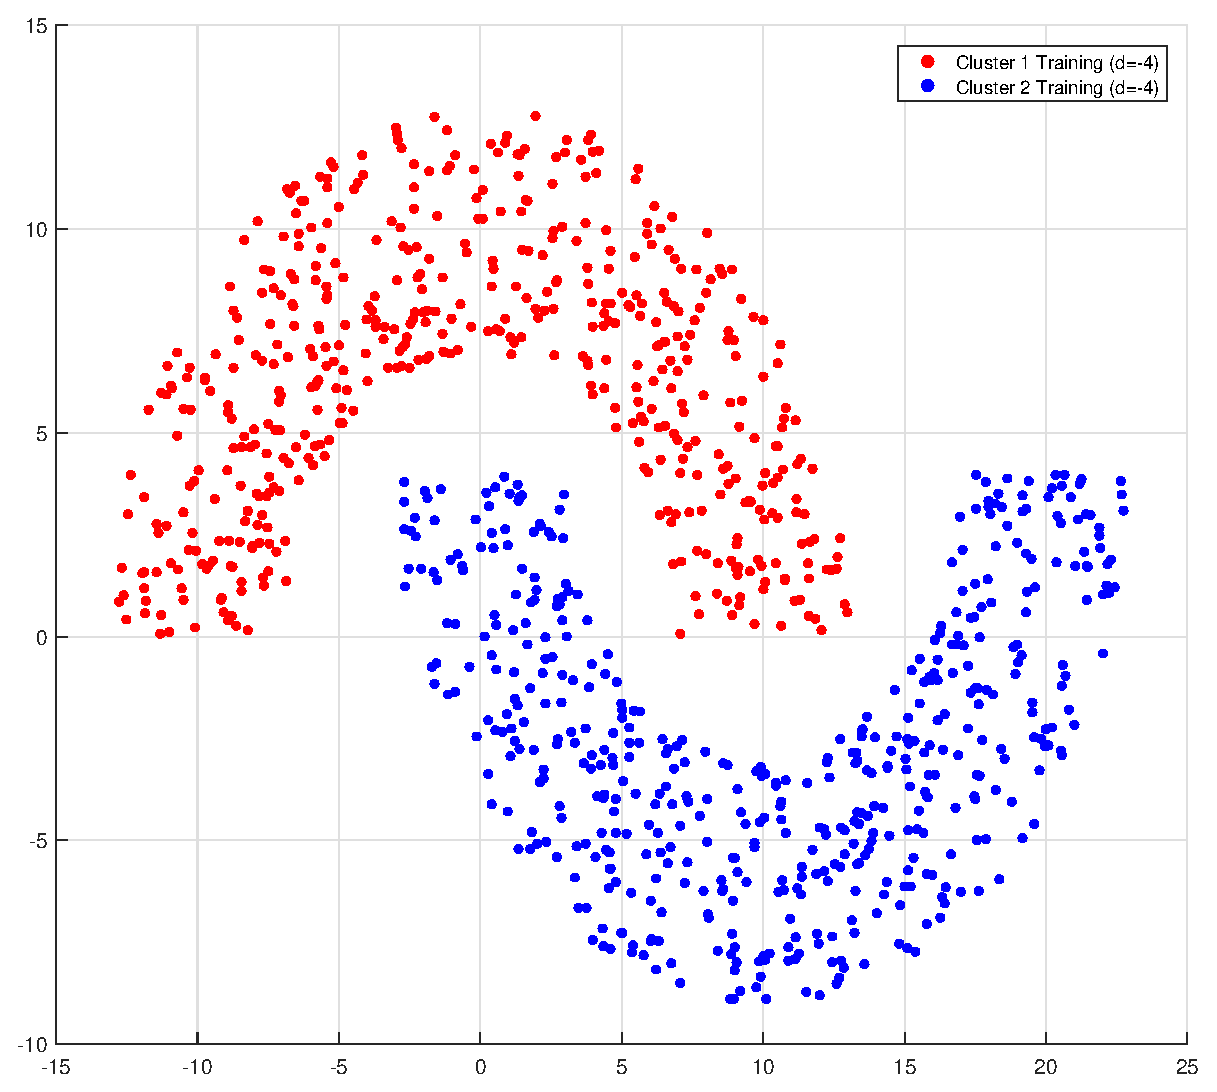
\includegraphics[width=3in,height=2in,clip,keepaspectratio]{ClustersDn4.eps} }\\
\caption{ Visualization of Clusters with separation of -4 units}
\end{figure}

\begin{figure}
\centering
{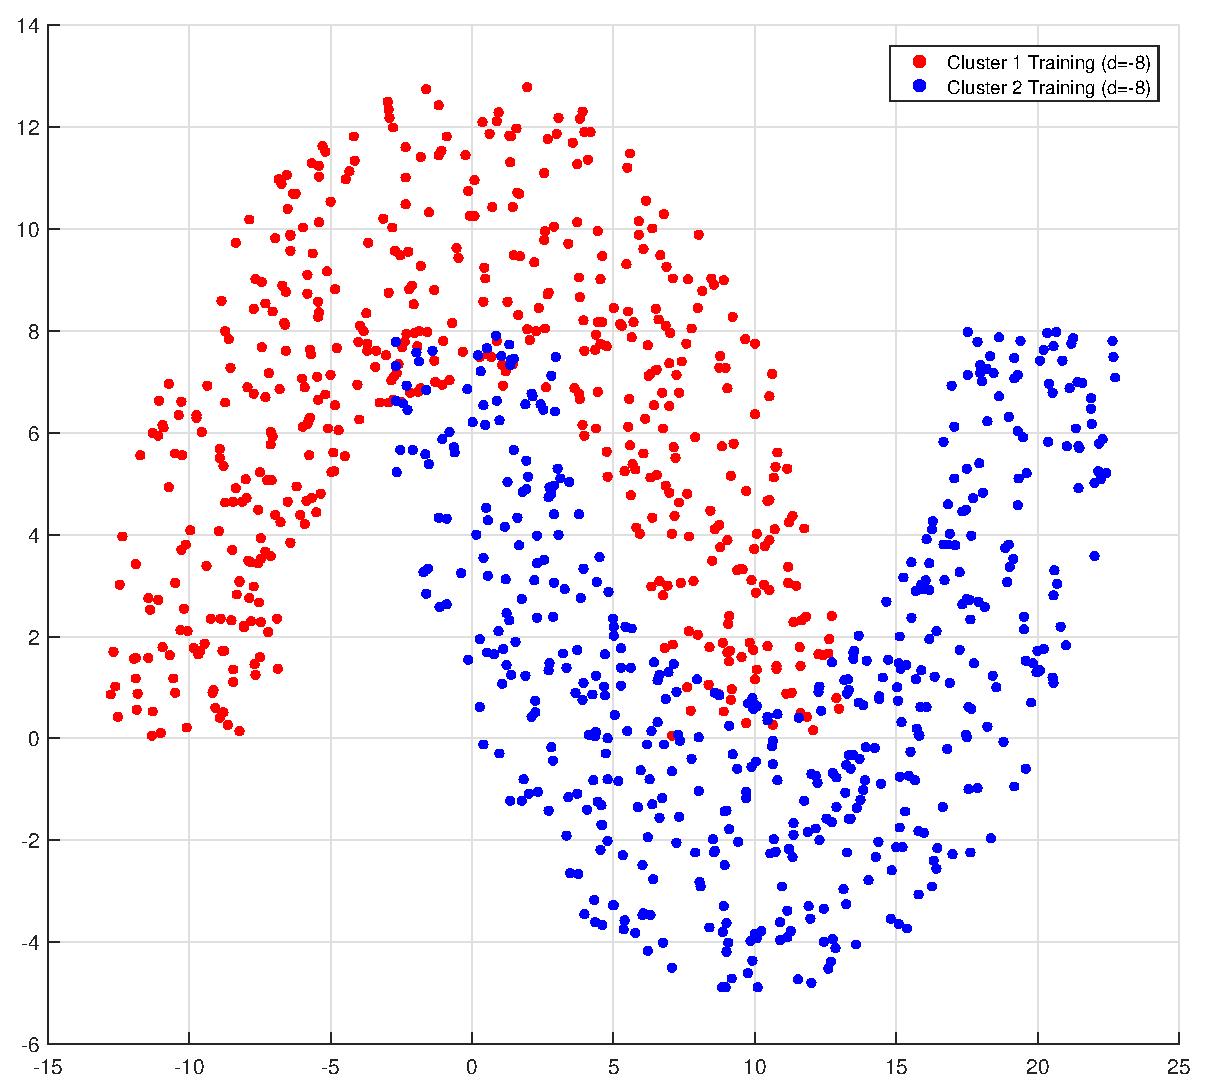
\includegraphics[width=3in,height=2in,clip,keepaspectratio]{ClustersDn8.eps} }\\
\caption{ Visualization of Clusters with separation of -8 units}
\end{figure}
\subsection{Training Data}
Initially, we have three layer neural net with first layer as input layer , second layer as hidden layer and third as output layer. Basically, we have single hidden layer with multiple neural units. As we are planning on designing the non linear classifier with data distribution as shown in fig. 1:3. We have trained network using different function available in MATLAB neural net toolbox  such as for basic back propagation we have used 'traingd' (Gradient Descend Back Propagation)\cite{gd} \cite{mgd}, for back propagation with momentum we have used 'trainrp' (Resilient Back Propagation Algorithm )\cite{gdm} \cite{mgdm}and for Levenberg Marquardt we have used 'trainlm' (Levenberg Marquardt )\cite{lm} \cite{mlm}. In this case, we have set the 75\% of data is training data and 25\% is used for cross validation. Furthermore, We have trained network with different learning rates having values viz. 1.6,0.9 and 0.2  for all three separation distances of 2, -4, -8.

\subsection{Testing Data}
 Here, we have generated 1000 testing data points for separation distant between clusters as d=2, d=-4 and d=-8. Here, visualization of trained neural network for different settings and parameter values is done in terms of decision boundary and learning curves. Lets Consider each algorithm for network training and its response to the  testing data.
\subsection{Experiment I}
\subsubsection{Basic Back Propagation}
 Now consider simple back propagation algorithm, we are using 'traingd'( Gradient Descend Algorithm)\cite{mgd} available in MATLAB Neural Net toolbox \cite{bpm}. we have set the number of units in hidden layer to 3. Here, we can visualize the response of single hidden layer neural network trained with different learning rates in fig. 4:9.
 \\
\subsubsection{Back Propagation with Momentum}
Here, We are using resilient back propagation algorithm available in MATLAB Neural Net tool box. Important parameter that we have to focused on is momentum rate of back propagation algorithm\cite{gdm} \cite{mgdm}. Due to addition of momentum rate, there is attenuation in oscillation of gradient descent \cite{gdm} . thus, we have tested the output of neural network trained with back propagation algorithm having momentum rate of "0.9" and response can be visulaized in terms of decision boundary in fig. 4:9\\

\subsubsection{Levenberg-Marquardt Back Propagation}
Levenberg Marquardt Back Propagation is optimal algorithm for least square estimation when we deal with non linear decision boundaries\cite{lm}. as per the given problem, we have used 'trainlm' (Levenberg Marquardt ) \cite{mlm} parameter available in MATLAB neural net tool box. Response of neural net with  Levenberg-Marquardt algorithm can be in fig. 4:9.

\subsection{Experiment II}
{ Initially we trained neural network with single hidden layer with three different back propagation algorithm and learning rates. however, in this part of experiment, we are restricting data set to cluster with separation distance of -8.Untill now, we have not changed the number of units (neurons) in hidden layers which indirectly was restriction on performance of neural network to complext data set (d=-8). But by changing  number of  units in hidden layer to 2, 5 and 11 we can visualize the change and improvement in performance using learning curves and decision boundaries shown in fig. 10 and fig. 11   }
\FloatBarrier
\section{Results}
\begin{figure}[h!]
\centering
{\includegraphics[width=3in,height=2in,clip,keepaspectratio]{Exp1_DB2.eps} }\\
\caption{Response of Neural Network in terms of decision boundary for cluster with separation distance of 2 units }
\end{figure}
\begin{figure}[h!]
\centering
{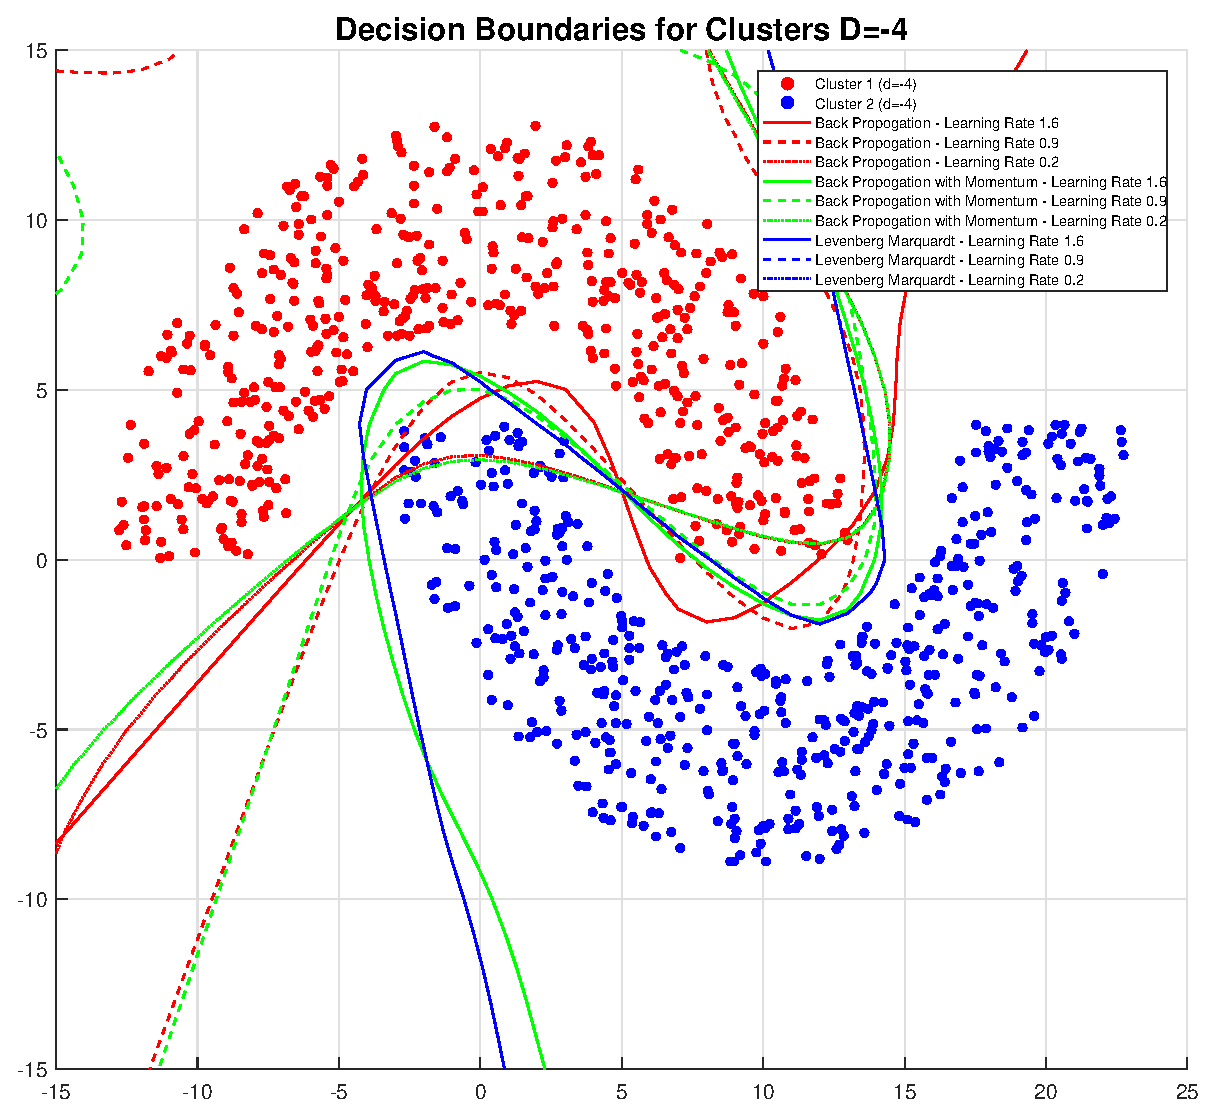
\includegraphics[width=3in,height=2in,clip,keepaspectratio]{Exp1_DBn4.eps} }\\
\caption{Response of Neural Network in terms of decision boundary for cluster with separation distance of -4 units}
\end{figure}
\begin{figure}[h!]
\centering
{\includegraphics[width=3in,height=2in,clip,keepaspectratio]{Exp1_DBn8.eps} }\\
\caption{Response of Neural Network in terms of decision boundary for cluster with separation distance of -8 units}
\end{figure}
\begin{figure}
\centering
{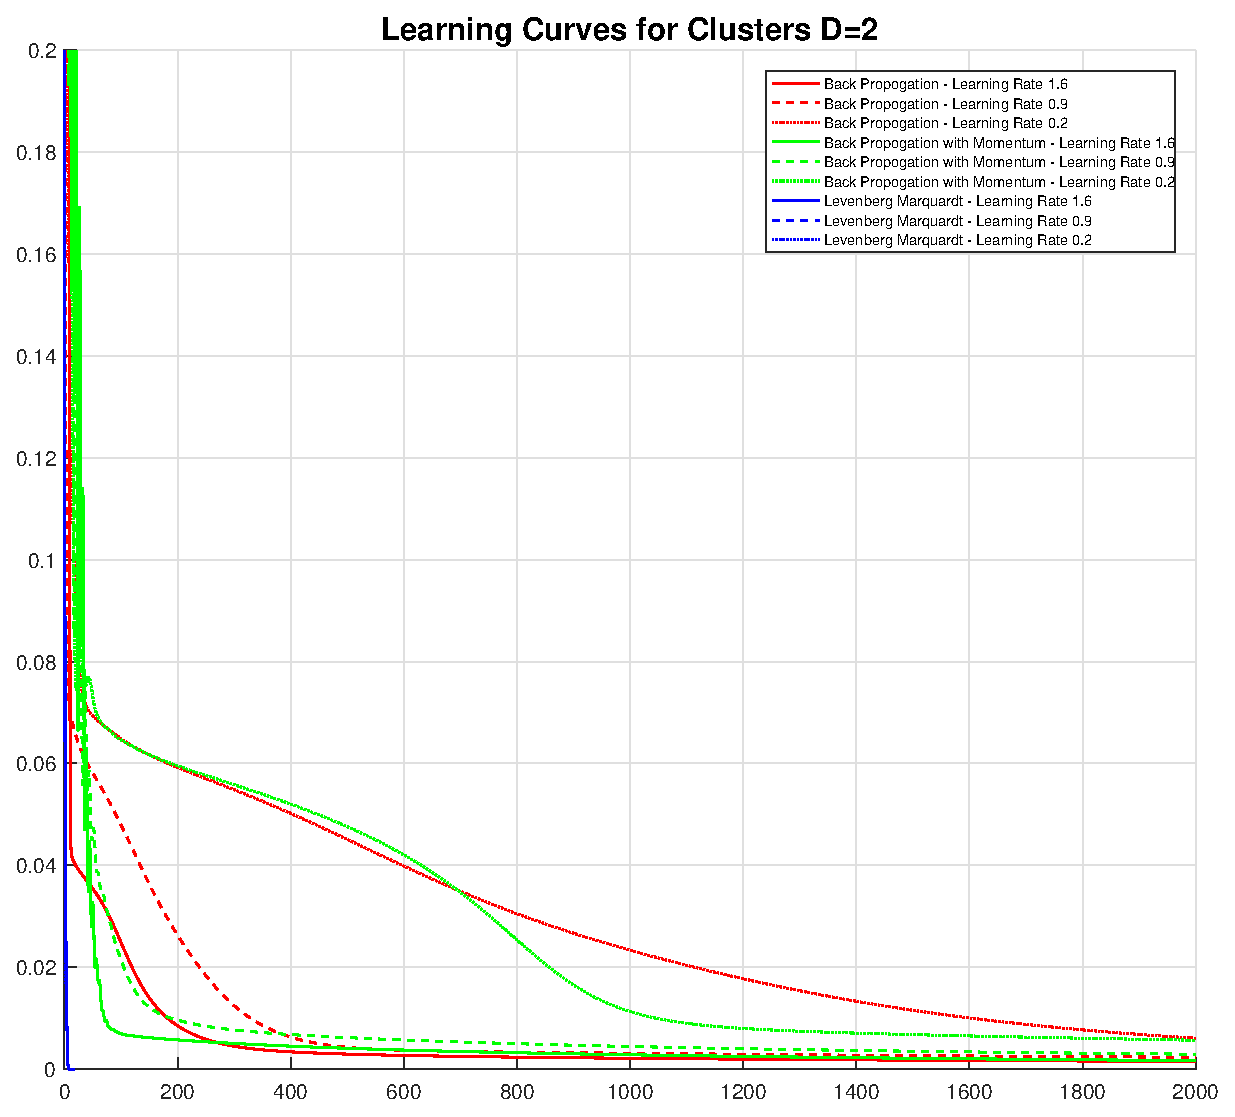
\includegraphics[width=3in,height=2in,clip,keepaspectratio]{Exp1_LC2.eps} }
\caption{Performance of three different algorithms for three different learning rates in terms of Learning Curve for data set with separation distance of 2 units }
\end{figure}
\begin{figure}
\centering
{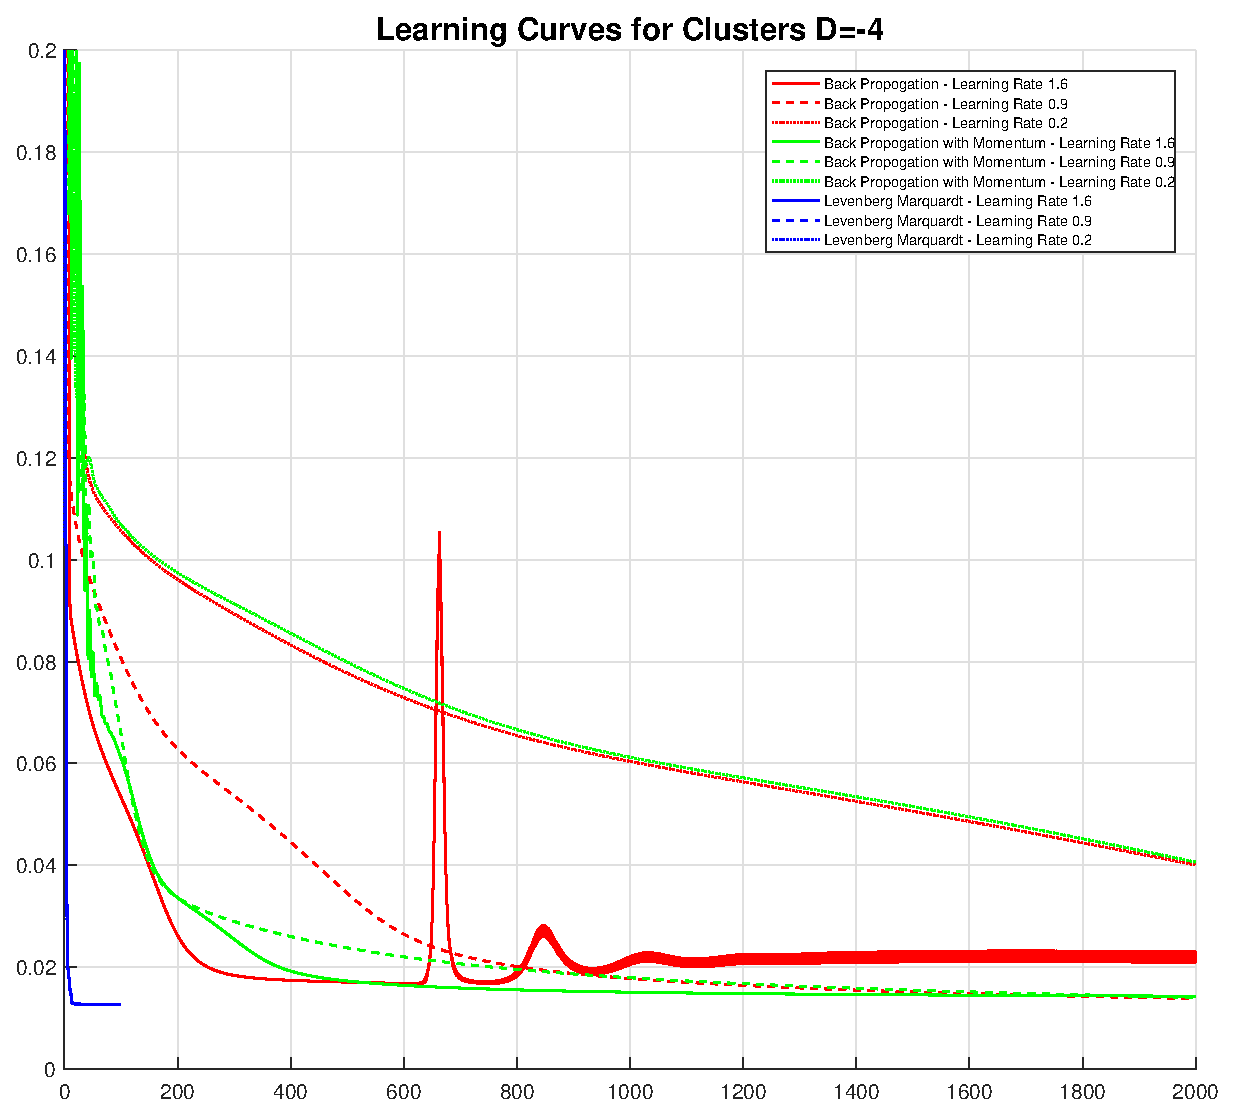
\includegraphics[width=3in,height=2in,clip,keepaspectratio]{Exp1_LCn4.eps} }\\
\caption{Performance of three different algorithms for three different learning rates in terms of Learning Curve for data set with separation distance of 2 units}
\end{figure}
\begin{figure}
\centering
{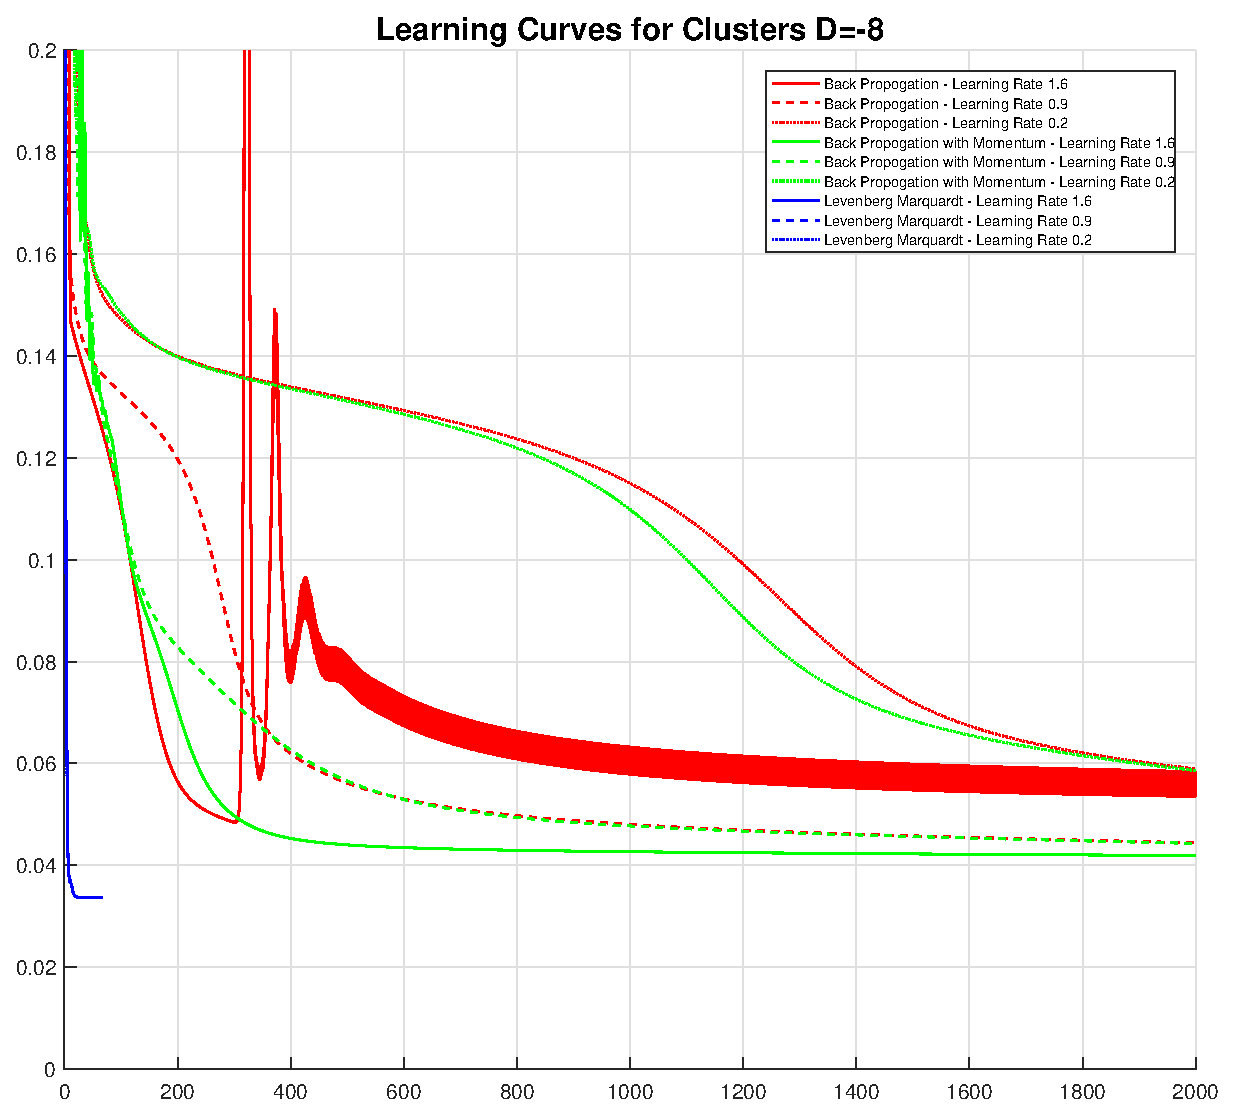
\includegraphics[width=3in,height=2in,clip,keepaspectratio]{Exp1_LCn8.eps} }\\
\caption{Performance of three different algorithms for three different learning rates in terms of Learning Curve for data set with separation distance of 2 units}
\end{figure}
\begin{figure}
\centering
{\includegraphics[width=3in,height=2in,clip,keepaspectratio]{Exp2_DBn8.eps} }\\
\caption{Response of Neural Network in terms of decision boundary  and different numbers of neurons for cluster with separation distance of -8 units}
\end{figure}
\begin{figure}
\centering
{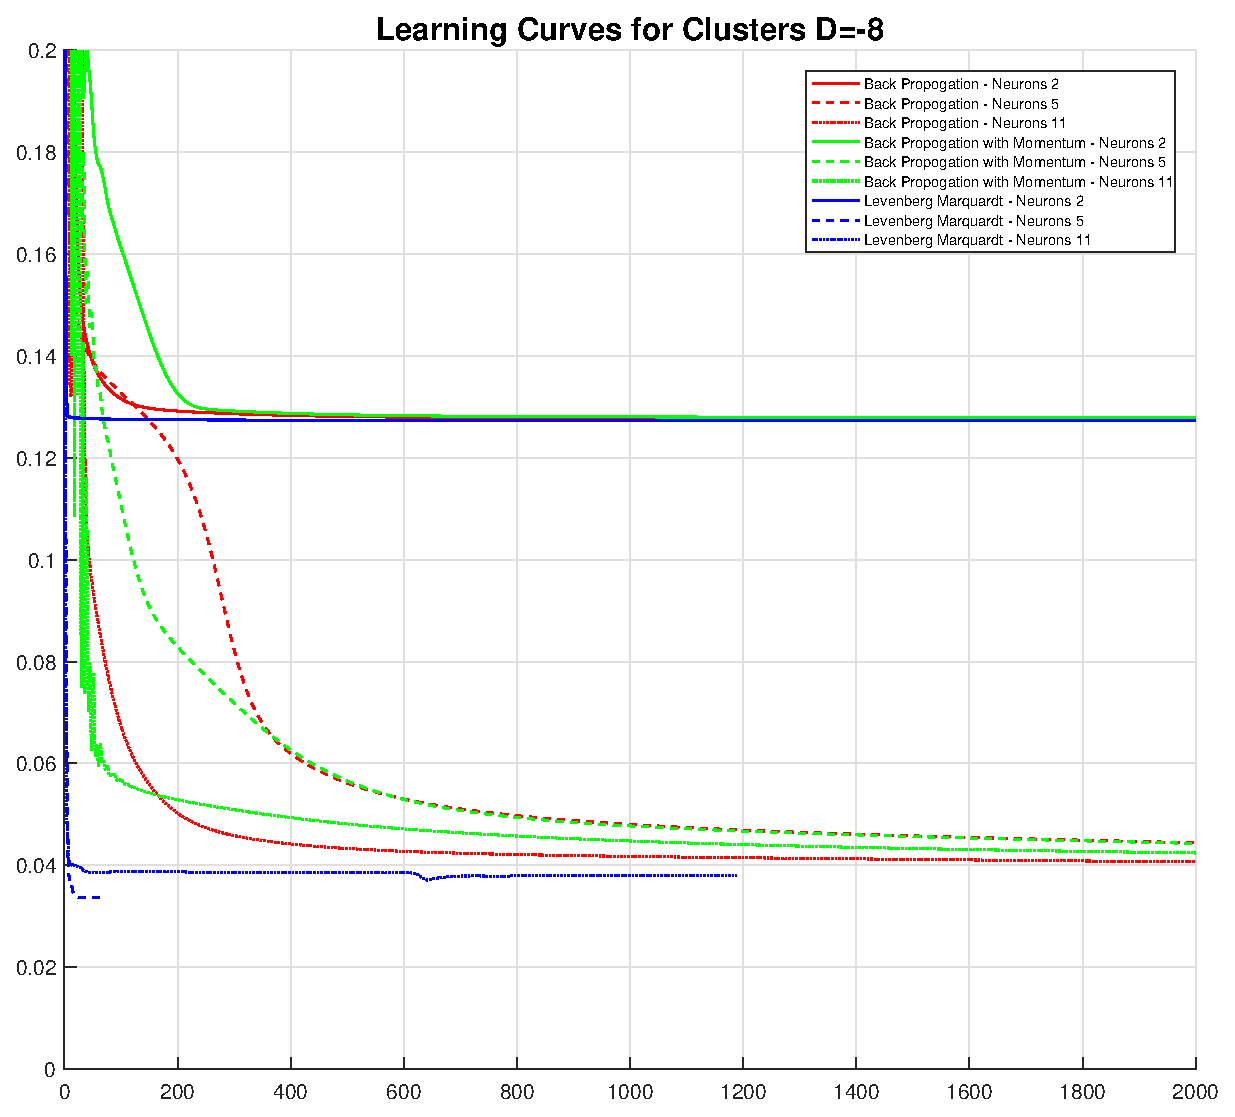
\includegraphics[width=3in,height=2in,clip,keepaspectratio]{Exp2_LCn8.eps} }\\
\caption{Performance of neural network with threedifferent algorithms and three different number of hiddenneurons in terms of Learning Curve for data set withseparation distance of -8 units }
\end{figure}
\begin{figure}
\centering
{\includegraphics[width=3in,height=2in,clip,keepaspectratio]{Confusion_Matrix_Summary_d2.png} }\\
\caption{Confusion Matrix Summary of Clusters with Separation distance d= 2 for different conditions}
\end{figure}
\begin{figure}
\centering
{\includegraphics[width=3in,height=2in,clip,keepaspectratio]{Confusion_Matrix_Summary_d4.png} }\\
\caption{Confusion Matrix Summary of Clusters with Separation distance d= -4 for different conditions}
\end{figure}
\begin{figure}
\centering
{\includegraphics[width=3in,height=2in,clip,keepaspectratio]{Confusion_Matrix_Summary_d8.png} }\\
\caption{Confusion Matrix Summary of Clusters with Separation distance d= -8 for different conditions}
\end{figure}

\section{Conclusion}

From this project, we understood how to implement back propagation algorithm and the merits and demerits of different algorithms such as back propagation with momentum and levenberg marquardt algorithm. A three layer neural network with enough neurons are enough to solve this classification problem but for even more complicated data sets which are not separable by a linear classifier, a more different sophisticated approach is required.
}


\bibliographystyle{IEEEtran}
\bibliography{references}
%\begin{thebibliography}{1}
%
%\bibitem{Multilayer Neural Networks and Back Propagation} 
%{Multilayer Neural Networks and Back Propagation }\\
% \url{https://www.mathworks.com/help/nnet/ug/multilayer-neural-networks-and-backpropagation-training.html}
% 
%\bibitem{}
%{Levenberg-Marquardt Algorithm}\\
%\url{https://www.mathworks.com/help/nnet/ref/trainlm.html}
%
%\bibitem{} 
%{Gradient Descend Back Propagation Algorithm}\\
%\url{}{https://www.mathworks.com/help/nnet/ref/traingd.html} 
%
%\bibitem{} {Resilient Back Propagation Algorithm}\\
%\url{https://www.mathworks.com/help/nnet/ref/trainrp.html}
%\bibitem{} 
%{Hugo Larochelle - Back Propagation}\\
%\url{https://www.youtube.com/watch?v=_KoWTD8T45Q&list=PL6Xpj9I5qXYEcOhn7TqghAJ6NAPrNmUBH&index=13} 
%
%\end{thebibliography}

\end{document}

